\section{Covariate Displacement and the Wasserstein Distance}\label{sec:appendix:zdisplacement}

This appendix formalizes the notion of covariate displacement for a linear estimator of a convex weighted average treatment effect and connects it to the Wasserstein-1 distance between the weighted covariate distributions on the treated and control sides.

\subsection{Setup}\label{sec:appendix:zdisplacement:setup}

Consider a linear estimator $\hat{\tau} = \sum_{i=1}^n w_i Y_i$ targeting a convex weighted average treatment effect $\tau_w = \sum_i \lambda_i \tau(c, Z_i)$ under the fixed-design framework of \cref{sec:setup}.
The weights satisfy $\sum_{i \in T} w_i = 1$ and $\sum_{i \in C} w_i = -1$, where $T = \{i : X_i \geq c\}$ and $C = \{i : X_i < c\}$ denote the treated and control groups.
For exposition, suppose first that all treated weights are non-negative and all control weights are non-positive.
Write $w_i^+ = w_i$ for $i \in T$ and $w_j^- = \abs{w_j}$ for $j \in C$, so that $\hat{\tau} = \sum_{i \in T} w_i^+ Y_i - \sum_{j \in C} w_j^- Y_j$ with $\sum_{i \in T} w_i^+ = \sum_{j \in C} w_j^- = 1$.
This sign convention holds for local constant estimators, including the segmented estimator of \cref{sec:setup:segmented}; the extension to general linear estimators with possibly negative weights is given in \cref{sec:appendix:zdisplacement:kr}.

The estimator implicitly compares treated and control units.
When a treated unit at $Z_i$ is effectively compared against a control unit at $Z_j \neq Z_i$, the comparison traverses a distance $\abs{Z_i - Z_j}$ in the covariate direction.
Under a Lipschitz bound $M_z$ in the $z$-direction, this displacement contributes up to $M_z \abs{Z_i - Z_j}$ to the worst-case bias.
The question is: what is the total covariate displacement induced by a given set of weights?

\subsection{Motivating Example}\label{sec:appendix:zdisplacement:example}

Consider a balanced design with two treated and two control units, all with equal weight $1/2$.
\Cref{fig:displacement_scenarios} illustrates the two scenarios.

\begin{figure}[ht]
\centering
\begin{subfigure}[b]{0.47\textwidth}
\centering
\begin{tikzpicture}[scale=0.85,
	treat/.style={fill=red!70!black, circle, inner sep=0pt, minimum size=6pt},
	ctrl/.style={fill=blue!70!black, circle, inner sep=0pt, minimum size=6pt},
	matchgood/.style={->, thick, green!50!black, shorten <=3pt, shorten >=3pt},
	]
	% cutoff
	\draw[dashed, gray!70, line width=0.8pt] (0,-0.3) -- (0,4.8);
	\node[above, gray!70, font=\footnotesize] at (0,4.8) {$c$};
	% axes
	\draw[->] (-3,-0.3) -- (3,-0.3) node[right, font=\footnotesize] {$X$};
	\draw[->] (-3,-0.3) -- (-3,4.8) node[above, font=\footnotesize] {$Z$};
	% Z ticks
	\foreach \z in {1,2,3,4} {
		\draw (-3,\z) -- +(-0.08,0) node[left, font=\footnotesize] {$\z$};
		\draw[dotted, gray!30] (-2.9,\z) -- (2.9,\z);
	}
	% side labels
	\node[font=\footnotesize, blue!70!black] at (-1.5,-0.7) {Control};
	\node[font=\footnotesize, red!70!black] at (1.5,-0.7) {Treated};
	% control units
	\node[ctrl] (c1) at (-1.3,1) {};
	\node[ctrl] (c3) at (-1.3,3) {};
	\node[left, font=\scriptsize] at (-1.55,1) {$\tfrac{1}{2}$};
	\node[left, font=\scriptsize] at (-1.55,3) {$\tfrac{1}{2}$};
	% treated units
	\node[treat] (t1) at (1.3,1) {};
	\node[treat] (t3) at (1.3,3) {};
	\node[right, font=\scriptsize] at (1.55,1) {$\tfrac{1}{2}$};
	\node[right, font=\scriptsize] at (1.55,3) {$\tfrac{1}{2}$};
	% matching arrows (horizontal = zero displacement)
	\draw[matchgood] (c1) -- (t1);
	\draw[matchgood] (c3) -- (t3);
	% displacement annotation
	\node[font=\footnotesize, green!50!black] at (0,0.55) {$\abs{\Delta Z} = 0$};
	\node[font=\footnotesize, green!50!black] at (0,2.55) {$\abs{\Delta Z} = 0$};
	% total
	\node[font=\small, anchor=north] at (0,-1.2) {$D_Z = 0$};
\end{tikzpicture}
\caption{Exact $Z$-balance: each treated unit has a control unit at the same covariate value.}
\label{fig:scenario1}
\end{subfigure}
\hfill
\begin{subfigure}[b]{0.47\textwidth}
\centering
\begin{tikzpicture}[scale=0.85,
	treat/.style={fill=red!70!black, circle, inner sep=0pt, minimum size=6pt},
	ctrl/.style={fill=blue!70!black, circle, inner sep=0pt, minimum size=6pt},
	matchbad/.style={->, thick, orange!80!black, shorten <=3pt, shorten >=3pt},
	]
	% cutoff
	\draw[dashed, gray!70, line width=0.8pt] (0,-0.3) -- (0,4.8);
	\node[above, gray!70, font=\footnotesize] at (0,4.8) {$c$};
	% axes
	\draw[->] (-3,-0.3) -- (3,-0.3) node[right, font=\footnotesize] {$X$};
	\draw[->] (-3,-0.3) -- (-3,4.8) node[above, font=\footnotesize] {$Z$};
	% Z ticks
	\foreach \z in {1,2,3,4} {
		\draw (-3,\z) -- +(-0.08,0) node[left, font=\footnotesize] {$\z$};
		\draw[dotted, gray!30] (-2.9,\z) -- (2.9,\z);
	}
	% side labels
	\node[font=\footnotesize, blue!70!black] at (-1.5,-0.7) {Control};
	\node[font=\footnotesize, red!70!black] at (1.5,-0.7) {Treated};
	% control units
	\node[ctrl] (c2) at (-1.3,2) {};
	\node[ctrl] (c3) at (-1.3,3) {};
	\node[left, font=\scriptsize] at (-1.55,2) {$\tfrac{1}{2}$};
	\node[left, font=\scriptsize] at (-1.55,3) {$\tfrac{1}{2}$};
	% treated units
	\node[treat] (t1) at (1.3,1) {};
	\node[treat] (t4) at (1.3,4) {};
	\node[right, font=\scriptsize] at (1.55,1) {$\tfrac{1}{2}$};
	\node[right, font=\scriptsize] at (1.55,4) {$\tfrac{1}{2}$};
	% matching arrows (diagonal = displacement)
	\draw[matchbad] (c2) -- (t1);
	\draw[matchbad] (c3) -- (t4);
	% displacement braces
	\draw[decorate, decoration={brace, amplitude=4pt, mirror}, orange!80!black]
		(1.7,1) -- (1.7,2) node[midway, right=5pt, font=\scriptsize, orange!80!black] {$\abs{\Delta Z} = 1$};
	\draw[decorate, decoration={brace, amplitude=4pt}, orange!80!black]
		(-1.7,3) -- (-1.7,4) node[midway, left=5pt, font=\scriptsize, orange!80!black] {$\abs{\Delta Z} = 1$};
	% total
	\node[font=\small, anchor=north] at (0,-1.2) {$D_Z = \tfrac{1}{2}\cdot 1 + \tfrac{1}{2}\cdot 1 = 1$};
\end{tikzpicture}
\caption{$Z$-imbalance: closest-pair matching still incurs displacement.  Both scenarios have identical mean balance.}
\label{fig:scenario2}
\end{subfigure}
\caption{Two designs with equal mean covariate balance $\sum_{i \in T} w_i^+ Z_i = \sum_{j \in C} w_j^- Z_j = 2$, but different covariate displacement.  Arrows indicate the optimal matching of treated to control units in the $Z$-dimension.}
\label{fig:displacement_scenarios}
\end{figure}

\paragraph{Scenario~1: Exact $Z$-balance.}
Let the control units have $Z$-values $\{1, 3\}$ and the treated units have $Z$-values $\{1, 3\}$.
With equal weights, the estimator computes
\begin{equation*}
	\hat{\tau} = \tfrac{1}{2}\bigl[m(3) - m(2)\bigr] + \tfrac{1}{2}\bigl[m(2) - m(3)\bigr],
\end{equation*}
where $m$ denotes the regression function restricted to the $z$-dimension (suppressing the $x$-argument, which is common to all comparisons at the cutoff).
This cross-comparison cancels exactly: the $Z$-displacement is zero.

\paragraph{Scenario~2: $Z$-imbalance.}
Now let the control units have $Z$-values $\{2, 3\}$ and the treated units $\{1, 4\}$.
The cross-comparison becomes
\begin{equation}\label{eq:cross_comparison}
	\hat{\tau} = \tfrac{1}{2}\bigl[m(4) - m(2)\bigr] + \tfrac{1}{2}\bigl[m(1) - m(3)\bigr].
\end{equation}
Applying the fundamental theorem of calculus:
\begin{align}
	\hat{\tau} &= \tfrac{1}{2}\int_2^4 m'(s)\, ds - \tfrac{1}{2}\int_1^3 m'(s)\, ds \notag \\
	&= \tfrac{1}{2}\left(\int_2^4 m'(s)\, ds - \int_1^3 m'(s)\, ds\right). \label{eq:cross_integrals}
\end{align}
The two integrals overlap on $[2,3]$, so the overlapping contributions cancel and only the non-overlapping parts survive:
\begin{equation}\label{eq:residual_displacement}
	\hat{\tau} = \tfrac{1}{2}\left(\int_3^4 m'(s)\, ds + \int_1^2 m'(s)\, ds\right).
\end{equation}
This residual is exactly what one would obtain by directly comparing the closest pairs: treated unit at $Z = 4$ against control at $Z = 3$ (displacement $1$), and treated at $Z = 1$ against control at $Z = 2$ (displacement $1$).
The total displacement is $\tfrac{1}{2} \cdot 1 + \tfrac{1}{2} \cdot 1 = 1$.

Under a Lipschitz bound $\abs{m'(z)} \leq M_z$, the worst-case bias from the covariate displacement in \eqref{eq:residual_displacement} is bounded by $M_z$ times the total displacement.
The key observation is that mean covariate balance ($\sum_{i \in T} w_i^+ Z_i = \sum_{j \in C} w_j^- Z_j$) does not capture this displacement: both scenarios have balanced means, yet Scenario~2 has positive displacement while Scenario~1 has none.


\subsection{Covariate Displacement via Optimal Transport}\label{sec:appendix:zdisplacement:transport}

The examples above suggest that the correct measure of covariate displacement is not a moment condition on $Z$, but the total cost of transporting the weighted control distribution to match the weighted treated distribution in the $Z$-dimension.
This is precisely the Wasserstein-1 distance.

\begin{definition}[Covariate Displacement]\label{def:cov_displacement}
	Let $\mu_T = \sum_{i \in T} w_i^+ \delta_{Z_i}$ and $\mu_C = \sum_{j \in C} w_j^- \delta_{Z_j}$ denote the discrete probability measures on the treated and control covariate values, weighted by the estimator weights.
	The \emph{covariate displacement} of the estimator is the Wasserstein-1 distance
	\begin{equation}\label{eq:cov_displacement}
		D_Z(\hat{\tau}) \defeq W_1(\mu_T, \mu_C) = \inf_{\gamma \in \Gamma(\mu_T, \mu_C)} \sum_{i \in T} \sum_{j \in C} \gamma_{ij}\, \abs{Z_i - Z_j},
	\end{equation}
	where $\Gamma(\mu_T, \mu_C)$ is the set of couplings: nonnegative matrices $(\gamma_{ij})$ with $\sum_{j \in C} \gamma_{ij} = w_i^+$ for all $i \in T$ and $\sum_{i \in T} \gamma_{ij} = w_j^-$ for all $j \in C$.
\end{definition}

The covariate displacement has the following properties:
\begin{enumerate}
	\item $D_Z(\hat{\tau}) = 0$ if and only if $\mu_T = \mu_C$ (exact $Z$-balance in distribution, not just in mean).
	\item $D_Z(\hat{\tau}) \geq 0$, with equality characterizing designs where every treated unit is compared against control units at the same covariate value.
	\item Under a Lipschitz bound $\abs{\partial m / \partial z} \leq M_z$, the worst-case bias contribution from covariate displacement is bounded by $M_z \cdot D_Z(\hat{\tau})$.
\end{enumerate}


\subsection{Closed-Form in One Dimension}\label{sec:appendix:zdisplacement:closedform}

For a scalar covariate $Z \in \mathbb{R}$, the Wasserstein-1 distance admits a closed-form expression in terms of the weighted cumulative distribution functions.
Define the weighted empirical CDFs
\begin{equation}\label{eq:weighted_cdfs}
	F_T(z) \defeq \sum_{i \in T} w_i^+\, \ind\{Z_i \leq z\}, \qquad F_C(z) \defeq \sum_{j \in C} w_j^-\, \ind\{Z_j \leq z\}.
\end{equation}
Then the covariate displacement is
\begin{equation}\label{eq:wasserstein_cdf}
	D_Z(\hat{\tau}) = \int_{-\infty}^{\infty} \abs{F_T(z) - F_C(z)}\, dz.
\end{equation}
Since $F_T$ and $F_C$ are piecewise constant, the integral reduces to a finite sum over the intervals between consecutive order statistics of the pooled $Z$-values $\{Z_i\}_{i=1}^n$.
Let $z_{(1)} < z_{(2)} < \cdots < z_{(K)}$ denote the distinct pooled values.
Then
\begin{equation}\label{eq:wasserstein_sum}
	D_Z(\hat{\tau}) = \sum_{k=1}^{K-1} \abs{F_T(z_{(k)}) - F_C(z_{(k)})} \cdot (z_{(k+1)} - z_{(k)}).
\end{equation}

\Cref{fig:cdf_displacement} illustrates this for Scenario~2 from \cref{sec:appendix:zdisplacement:example}.
The treated CDF $F_T$ jumps at $Z = 1$ and $Z = 4$; the control CDF $F_C$ jumps at $Z = 2$ and $Z = 3$.
The shaded area between the two step functions equals $D_Z = 1$.

\begin{figure}[ht]
\centering
\begin{tikzpicture}[scale=1.1]
	% axes
	\draw[->] (-0.5,0) -- (5.8,0) node[right, font=\footnotesize] {$z$};
	\draw[->] (0,-0.15) -- (0,1.4) node[above, font=\footnotesize] {CDF};
	% y ticks
	\draw (0,0.5) -- +(-0.08,0) node[left, font=\footnotesize] {$\tfrac{1}{2}$};
	\draw (0,1.0) -- +(-0.08,0) node[left, font=\footnotesize] {$1$};
	\draw[dotted, gray!30] (0.05,0.5) -- (5.5,0.5);
	\draw[dotted, gray!30] (0.05,1.0) -- (5.5,1.0);
	% z ticks
	\foreach \z in {1,2,3,4,5} {
		\draw (\z,-0.05) -- (\z,0.05) node[below=2pt, font=\footnotesize] {$\z$};
	}
	%
	% Shaded area |F_T - F_C| FIRST (behind the lines)
	% [1,2): F_T = 1/2, F_C = 0 => gap = 1/2
	\fill[orange!25] (1,0) rectangle (2,0.5);
	% [3,4): F_T = 1/2, F_C = 1 => gap = 1/2
	\fill[orange!25] (3,0.5) rectangle (4,1.0);
	%
	% F_T (red): 0 for z<1, 1/2 for 1<=z<4, 1 for z>=4
	\draw[red!70!black, very thick]
		(-0.3,0) -- (1,0)
		(1,0.5) -- (4,0.5)
		(4,1.0) -- (5.5,1.0);
	% jumps
	\draw[red!70!black, thick, dashed] (1,0) -- (1,0.5);
	\draw[red!70!black, thick, dashed] (4,0.5) -- (4,1.0);
	\fill[red!70!black] (1,0.5) circle (1.8pt);
	\fill[red!70!black] (4,1.0) circle (1.8pt);
	\draw[red!70!black] (1,0) circle (1.8pt);
	\draw[red!70!black] (4,0.5) circle (1.8pt);
	%
	% F_C (blue): 0 for z<2, 1/2 for 2<=z<3, 1 for z>=3
	\draw[blue!70!black, very thick]
		(-0.3,0) -- (2,0)
		(2,0.5) -- (3,0.5)
		(3,1.0) -- (5.5,1.0);
	% jumps
	\draw[blue!70!black, thick, dashed] (2,0) -- (2,0.5);
	\draw[blue!70!black, thick, dashed] (3,0.5) -- (3,1.0);
	\fill[blue!70!black] (2,0.5) circle (1.8pt);
	\fill[blue!70!black] (3,1.0) circle (1.8pt);
	\draw[blue!70!black] (2,0) circle (1.8pt);
	\draw[blue!70!black] (3,0.5) circle (1.8pt);
	%
	% Annotations
	\node[font=\scriptsize, orange!80!black] at (1.5,0.25) {$\tfrac{1}{2}$};
	\node[font=\scriptsize, orange!80!black] at (3.5,0.75) {$\tfrac{1}{2}$};
	%
	% Legend
	\draw[red!70!black, very thick] (4.3,1.35) -- (4.8,1.35) node[right, font=\footnotesize] {$F_T$};
	\draw[blue!70!black, very thick] (4.3,1.15) -- (4.8,1.15) node[right, font=\footnotesize] {$F_C$};
	%
	% Total displacement annotation
	\node[font=\footnotesize, anchor=west] at (5.0, 0.5) {$D_Z = \displaystyle\int \abs{F_T - F_C}\, dz = 1$};
\end{tikzpicture}
\caption{Covariate displacement as the area between weighted empirical CDFs (Scenario~2).  The treated CDF $F_T$ (red) jumps at $Z \in \{1,4\}$; the control CDF $F_C$ (blue) jumps at $Z \in \{2,3\}$.  The shaded area equals the Wasserstein-1 distance $D_Z = 1$.}
\label{fig:cdf_displacement}
\end{figure}


\subsection{Greedy Matching Algorithm}\label{sec:appendix:zdisplacement:algorithm}

The optimal transport plan in one dimension can be computed by a greedy algorithm that processes units in order of their $Z$-values.
Since the optimal coupling for scalar measures is the monotone coupling (matching quantile functions), sorting and sequentially matching weight from one end yields the minimum-cost plan.

\paragraph{Algorithm.}
Sort all units by $Z_i$.
Process them from smallest to largest $Z$.
For each unit $i$, find the closest available unit $j$ on the opposite side of the cutoff (in the $Z$-dimension).
\begin{enumerate}
	\item Compute the weight difference $\Delta = w_i^{\mathrm{res}} - w_j^{\mathrm{res}}$, where $w^{\mathrm{res}}$ denotes residual (unmatched) weight.
	\item Match weight $\gamma_{ij} = \min(w_i^{\mathrm{res}},\, w_j^{\mathrm{res}})$ and record displacement $d_{ij} = \gamma_{ij}\, \abs{Z_i - Z_j}$.
	\item Update residual weights: if $\Delta = 0$, both units are fully matched and we proceed to the next pair; if $\Delta > 0$, unit $i$ retains residual weight $\Delta$ and seeks the next-closest match; if $\Delta < 0$, unit $j$ retains residual weight $\abs{\Delta}$ and continues matching to subsequent units.
\end{enumerate}
The total covariate displacement is
\begin{equation}\label{eq:greedy_displacement}
	D_Z(\hat{\tau}) = \sum_{\text{matched pairs } (i,j)} d_{ij}.
\end{equation}
This algorithm produces the same value as the closed-form \eqref{eq:wasserstein_sum} and runs in $O(n \log n)$ time (dominated by the initial sort).

\Cref{fig:greedy_matching} illustrates the algorithm for a design with unequal weights.
Three control units at $Z \in \{1, 3, 5\}$ with weights $(\tfrac{1}{4}, \tfrac{1}{2}, \tfrac{1}{4})$ are matched against two treated units at $Z \in \{2, 4\}$ with weights $(\tfrac{1}{2}, \tfrac{1}{2})$.
Processing from bottom to top: unit $C_1$ ($Z=1$, weight $\tfrac{1}{4}$) matches fully to $T_1$ ($Z=2$), transferring weight $\tfrac{1}{4}$ with displacement $1$.
The residual weight $\tfrac{1}{4}$ of $T_1$ then matches to $C_2$ ($Z=3$), displacement $1$.
The remaining weight $\tfrac{1}{4}$ of $C_2$ matches to $T_2$ ($Z=4$), displacement $1$.
Finally, $T_2$'s residual $\tfrac{1}{4}$ matches $C_3$ ($Z=5$), displacement $1$.
Total: $D_Z = 4 \times \tfrac{1}{4} \times 1 = 1$.

\begin{figure}[ht]
\centering
\begin{tikzpicture}[
	treat/.style={fill=red!70!black, circle, inner sep=0pt, minimum size=7pt},
	ctrl/.style={fill=blue!70!black, circle, inner sep=0pt, minimum size=7pt},
	marrow/.style={->, thick, shorten <=4pt, shorten >=4pt},
	wlabel/.style={font=\scriptsize, fill=white, inner sep=1pt},
	]
	% Z axis (horizontal)
	\draw[->] (-0.5,0) -- (7,0) node[right, font=\footnotesize] {$Z$};
	\foreach \z in {1,2,3,4,5,6} {
		\draw (\z,-0.08) -- (\z,0.08);
		\node[below=3pt, font=\footnotesize] at (\z,0) {$\z$};
	}
	%
	% Control units (below axis)
	\node[ctrl, label={[font=\scriptsize, blue!70!black]below:{$w^-\!=\!\tfrac{1}{4}$}}] (c1) at (1,-0.8) {};
	\node[ctrl, label={[font=\scriptsize, blue!70!black]below:{$w^-\!=\!\tfrac{1}{2}$}}] (c2) at (3,-0.8) {};
	\node[ctrl, label={[font=\scriptsize, blue!70!black]below:{$w^-\!=\!\tfrac{1}{4}$}}] (c3) at (5,-0.8) {};
	\node[font=\footnotesize, blue!70!black] at (-0.3,-0.8) {$C$};
	%
	% Treated units (above axis)
	\node[treat, label={[font=\scriptsize, red!70!black]above:{$w^+\!=\!\tfrac{1}{2}$}}] (t1) at (2,0.8) {};
	\node[treat, label={[font=\scriptsize, red!70!black]above:{$w^+\!=\!\tfrac{1}{2}$}}] (t2) at (4,0.8) {};
	\node[font=\footnotesize, red!70!black] at (-0.3,0.8) {$T$};
	%
	% Matching arrows with transferred weight
	% Step 1: C1 -> T1, weight 1/4
	\draw[marrow, green!50!black] (c1) -- (t1) node[wlabel, midway, left=1pt] {$\tfrac{1}{4}$};
	% Step 2: T1 -> C2, weight 1/4 (residual of T1)
	\draw[marrow, orange!80!black] (t1) -- (c2) node[wlabel, midway, left=1pt] {$\tfrac{1}{4}$};
	% Step 3: C2 -> T2, weight 1/4 (residual of C2)
	\draw[marrow, green!50!black] (c2) -- (t2) node[wlabel, midway, left=1pt] {$\tfrac{1}{4}$};
	% Step 4: T2 -> C3, weight 1/4 (residual of T2)
	\draw[marrow, orange!80!black] (t2) -- (c3) node[wlabel, midway, left=1pt] {$\tfrac{1}{4}$};
	%
	% Step numbers
	\node[font=\tiny, gray] at (1.3, 0.25) {\textcircled{1}};
	\node[font=\tiny, gray] at (2.7, 0.25) {\textcircled{2}};
	\node[font=\tiny, gray] at (3.3, 0.25) {\textcircled{3}};
	\node[font=\tiny, gray] at (4.7, 0.25) {\textcircled{4}};
	%
	% Total
	\node[font=\footnotesize, anchor=west] at (5.8, 0) {$D_Z = 4 \times \tfrac{1}{4} = 1$};
\end{tikzpicture}
\caption{Greedy matching algorithm with unequal weights.  Control units (blue, below) at $Z \in \{1,3,5\}$ are matched to treated units (red, above) at $Z \in \{2,4\}$.  Each arrow transfers the minimum of the two residual weights across a displacement of $\abs{\Delta Z} = 1$.  Arrows alternate direction as residual weight passes from one side to the other.}
\label{fig:greedy_matching}
\end{figure}


\subsection{Connection to Worst-Case Bias}\label{sec:appendix:zdisplacement:bias}

\subsubsection*{Non-Negative Weights}

When all estimator weights have the conventional sign --- positive for treated units, negative for control units --- the Wasserstein formulation of \cref{def:cov_displacement} applies directly.
In this case, the $z$-component of the worst-case bias under the separable Lipschitz class $\mathcal{F}_1^{\mathrm{aniso}}(M_x, M_z)$ satisfies
\begin{equation}\label{eq:bias_bound_z}
	\sup_{m \in \mathcal{F}_1^{\mathrm{aniso}}(M_x, M_z)} \abs{\text{Bias}_z(\hat{\tau})} \leq M_z \cdot D_Z(\hat{\tau}) = M_z \cdot W_1(\mu_T, \mu_C).
\end{equation}
This bound is tight: equality is attained by $m(x,z) = M_z \cdot z$.
Local constant estimators, including the segmented estimator of \cref{sec:setup:segmented}, always produce non-negative weights, so the Wasserstein interpretation applies to them without qualification.


\subsubsection*{The Negative Weights Problem}

Not all estimators have non-negative weights.
Local linear estimators, which are standard in RDD practice, assign negative weights to observations near the bandwidth boundary to correct for boundary bias.
More generally, minimax optimal estimators for higher-order smoothness classes can produce weights of either sign.
When a treated unit receives a negative weight, the measure $\mu_T = \sum_{i \in T} w_i^+ \delta_{Z_i}$ has negative mass and is no longer a probability measure, so the Wasserstein distance $W_1(\mu_T, \mu_C)$ is not defined.


\subsection{General Estimators and the Kantorovich--Rubinstein Norm}\label{sec:appendix:zdisplacement:kr}

The Kantorovich--Rubinstein (KR) duality provides a natural generalization that handles arbitrary weight signs.
The key observation is that the worst-case bias in the $z$-direction under the separable Lipschitz class \emph{is} a KR norm, without any assumption on the signs of the weights.

To see this, consider the one-sided problem: estimating the weighted average $\sum_k \lambda_k m(c, Z_k)$ from observations on the treated side using $\sum_{i \in T} w_i Y_i$.
The $z$-component of the bias, isolating the variation in $z$ at $x = c$, is
\begin{equation}\label{eq:bias_z_functional}
	\text{Bias}_z = \sum_{i \in T} w_i\, g(Z_i) - \sum_{k} \lambda_k\, g(Z_k)
\end{equation}
for a function $g : \mathcal{Z} \to \mathbb{R}$ with $\abs{g'} \leq M_z$.
Define the signed measure
\begin{equation}\label{eq:signed_measure}
	\nu \defeq \sum_{i \in T} w_i\, \delta_{Z_i} - \sum_{k} \lambda_k\, \delta_{Z_k},
\end{equation}
which has total mass zero (since $\sum_{i \in T} w_i = 1 = \sum_k \lambda_k$) and captures the discrepancy between the estimator's effective weighting over $Z$-values and the target weighting.
The worst-case bias in the $z$-direction is
\begin{equation}\label{eq:kr_bias}
	\sup_{\abs{g'} \leq 1} \left|\int g\, d\nu \right| \defeq \norm{\nu}_{KR},
\end{equation}
the Kantorovich--Rubinstein norm (also called the dual-Lipschitz norm) of $\nu$.
Scaling by $M_z$:
\begin{equation}\label{eq:bias_kr}
	\sup_{\abs{g'} \leq M_z} \abs{\text{Bias}_z} = M_z \cdot \norm{\nu}_{KR}.
\end{equation}
This holds for any linear estimator, regardless of the signs of the individual weights $w_i$.
The same argument applies to the control side, so the total $z$-displacement for the treatment effect estimator is the sum of the KR norms from the two one-sided problems.

\begin{remark}[Reduction to Wasserstein]\label{rem:kr_wasserstein}
	When all weights $w_i$ for $i \in T$ are non-negative, the signed measure decomposes as $\nu = \mu_{\hat{w}} - \mu_\lambda$ where both are probability measures: $\mu_{\hat{w}} = \sum_{i \in T} w_i \delta_{Z_i}$ and $\mu_\lambda = \sum_k \lambda_k \delta_{Z_k}$.
	In this case, $\norm{\nu}_{KR} = W_1(\mu_{\hat{w}}, \mu_\lambda)$, the Wasserstein-1 distance.
	When additionally the estimator targets $\tau(c)$ with $\lambda_k$ proportional to the control weights (i.e., matching treated against control), this recovers \cref{def:cov_displacement}.
	The KR norm is therefore the natural generalization of covariate displacement to estimators with negative weights.
\end{remark}

\begin{remark}[Computation]\label{rem:kr_computation}
	For a signed measure $\nu$ on $\mathbb{R}$ with total mass zero, the KR norm admits the closed-form
	\begin{equation}\label{eq:kr_cdf}
		\norm{\nu}_{KR} = \int_{-\infty}^{\infty} \abs{F_\nu(z)}\, dz,
	\end{equation}
	where $F_\nu(z) = \nu\bigl((-\infty, z]\bigr)$ is the signed cumulative distribution function.
	This generalizes \eqref{eq:wasserstein_cdf}: when $\nu = \mu_T - \mu_C$ with both measures being probability distributions, $F_\nu = F_T - F_C$ and the formula reduces to the CDF representation of $W_1$.
\end{remark}


\subsection{Bias Decomposition under Separability}\label{sec:appendix:zdisplacement:decomposition}

Under the separable class $\mathcal{F}_1^{\mathrm{aniso}}(M_x, M_z)$, the support function is $h_{\mathcal{C}}(\Delta x, \Delta z) = M_x \abs{\Delta x} + M_z \abs{\Delta z}$.
This additive structure means that the worst-case function can vary independently in $x$ and $z$.
On each side of the cutoff, the worst-case bias therefore decomposes into an $x$-component and a $z$-component:
\begin{equation}\label{eq:bias_decomposition}
	\wcb^{\pm}(\hat{\tau}_w) = M_x \cdot D_X^{\pm}(\hat{\tau}_w) + M_z \cdot D_Z^{\pm}(\hat{\tau}_w),
\end{equation}
where $D_X^{\pm}$ captures the displacement from the cutoff (the standard source of RDD bias) and $D_Z^{\pm} = \norm{\nu^{\pm}}_{KR}$ captures the covariate displacement as formalized in \cref{sec:appendix:zdisplacement:kr}, with $\nu^{\pm}$ denoting the signed measures on $Z$-values from the treated and control sides respectively.
The full worst-case bias of the treatment effect estimator is the sum of the two one-sided contributions.

This decomposition is a direct consequence of the product structure (separability) of the constraint set.
Under a coupled class such as the isotropic $\mathcal{F}_1^{\mathrm{iso}}(M)$, the support function is $h_{\mathcal{C}}(\Delta x, \Delta z) = M \norm{(\Delta x, \Delta z)}_2$, which does not decompose additively.
The $X$- and $Z$-contributions to bias are entangled, and the covariate displacement $D_Z$ cannot be read off separately.
This is a further advantage of the separable class: it makes the bias cost of $Z$-imbalance transparent and computable from the design alone.

\begin{remark}[Finite-sample diagnostic]\label{rem:diagnostic}
	The covariate displacement $D_Z(\hat{\tau}_w) = \norm{\nu}_{KR}$ provides a finite-sample, design-based diagnostic for the cost of $Z$-imbalance.
	Unlike mean balance conditions such as $\sum_i w_i Z_i = 0$, it captures the full distributional mismatch and cannot be fooled by symmetric imbalances that cancel in mean but incur real bias.
	It is computable from the observed $(X_i, Z_i, w_i)$ via \eqref{eq:kr_cdf} without knowledge of the unknown regression function.
\end{remark}
